\begin{figure}
    \begin{center}
        % 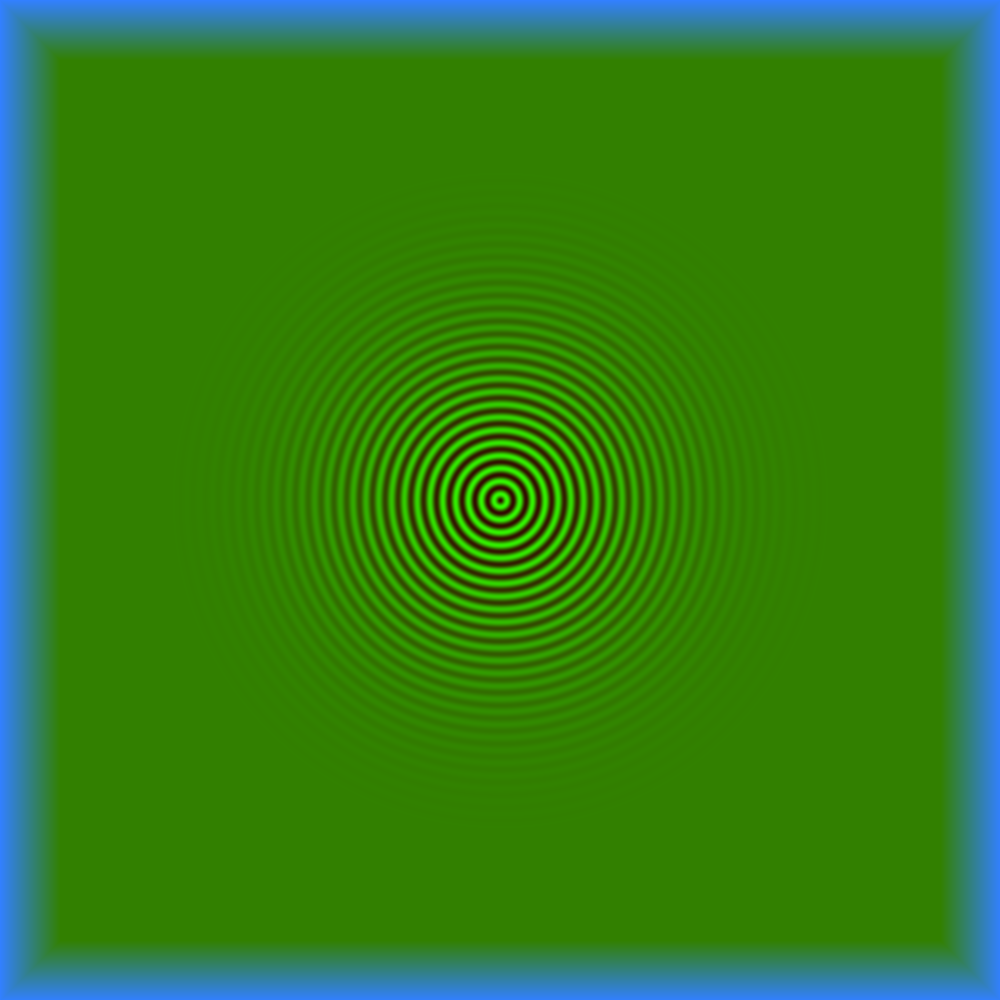
\includegraphics[width=0.5\textwidth]{papers/particles/figures/wavesim/particle_initial_state.png}
        \subfigure[0:08]{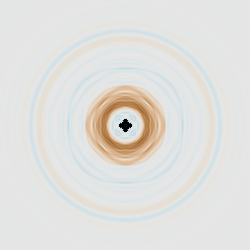
\includegraphics[width=0.49\textwidth]{papers/particles/figures/simulations/particle_frames/frame_02.png}\label{particles:fig:partikel:wachsen-1}}\hfill
        \subfigure[0:16]{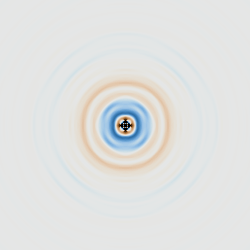
\includegraphics[width=0.49\textwidth]{papers/particles/figures/simulations/particle_frames/frame_04.png}\label{particles:fig:partikel:wachsen-2}}
        \caption{Feldkonfigurationen mit zunehmend wachsender Energieansammlung im Zentrum der Simulation und korrespondierenden Zeitstempeln aus dem Video \cite{particles:video-particle}.}\label{particles:fig:partikel:wachsen}
    \end{center}
\end{figure}
